\documentclass[Main.tex]{subfiles}
\begin{document}
\section{Probleemstelling}
Gebruikers hebben reeds de mogelijkheid om patroonherkenning te gebruiken op hun dataset. Toch kan de gebruiker op zoek zijn naar een wiskundige relatie in zijn dataset in plaats van een patroon. De hoofdhypothese van dit onderzoek is de volgende: \textbf{"Er kan voor een gegeven dataset binnen een beperkte tijd een passende vergelijking gevonden worden die voldoet aan de verwachtingen van de gebruiker."}. \\ \\
\newpage
\noindent
Gegeven: 
\begin{itemize}
\item Tabel T met kolommen $a_{1},\dotsc,a_{n},b$ 
	\begin{itemize}
	\item[$\rightarrow$] $e \in a_{1},\dotsc,a_{n}, b \Rightarrow e \in \mathbb{R}$
	\end{itemize}
\item Contextvrije grammatica G (Fig. \ref{fig:cfg})
\end{itemize}
Vind:
\begin{itemize}
\item Functie f in de taal van G zodat $f(a_{1}(i),\dotsc ,a_{n}(i)) = b(i)$ voor elke rij $i$ in T
\end{itemize}
\noindent
Dit proces moet gebeuren in een beperkte tijd. De oplossingsgraad van dit probleem is het percentage van tabellen waar er een geschikte functie, in de taal van de contextvrije grammatica, gevonden wordt. Met de term kolomwaarden wordt bedoeld: de waarden die door de gebruiker worden meegegeven verschillend van de oplossing. Deze worden in de voorbeelden aangegeven als $a$ en $b$.

\par De volgende subsecties geven de benodigde voorkennis weer voor het vervolg van de paper.

\subsection{Contextvrije grammatica}
Om wiskundige vergelijkingen op te bouwen wordt er gebruik gemaakt van een contextvrije grammatica (CFG) \cite{equationDisc}. Volgens de \textit{formele taal theorie} \cite{cfg} is een contextvrije grammatica een formele grammatica waarbij elke productieregel er uit ziet als volgt: $V \rightarrow w$. Hier staat $V$  voor \'e\'en niet-terminaal symbool en $w$ voor een tekenreeks van niet-terminale en terminale symbolen. Contextvrij betekent dat de productieregels kunnen toegepast worden los van de context waarin het niet-terminaal symbool zich bevindt.

\begin{figure}[!htb]
\centering
\begin{framed}
$E \rightarrow E + E$ \\
$E \rightarrow E - E$ \\
$E \rightarrow E \ast E$ \\
$E \rightarrow E \div E$ \\
$E \rightarrow E^{\wedge}E$ \\
$E \rightarrow a | b | \dotsc$
\end{framed}
\caption{De contextvrije grammatica}
\label{fig:cfg}
\end{figure}

Als een andere wiskundige operatie gewenst is, kan er een productieregel met deze operatie aan de bovenstaande grammatica worden toegevoegd. Voordelig aan het werken met een contextvrije grammatica is de gemakkelijke aanpasbaarheid. Omdat productieregels volledig onafhankelijk zijn van elkaar, is het eenvoudig om de gewenste operaties door de gebruiker te laten defini\"eren. In de voorbeelden die hierna zullen volgen wordt de grammatica uit Figuur \ref{fig:cfg} gebruikt. De productieregels die het algoritme bevat zijn: $+, -, \ast, \div$ en~\^{}.

\subsection{Boomstructuur}

Door de herhaaldelijke toepassing van de productieregels, met uitzondering van de productieregels die eindigen in terminale symbolen, onstaat er een boomstructuur. In deze boom bevinden zich alle mogelijke woorden die in de taal van de grammatica bepaald kunnen worden. Bij het opstellen van deze boom wordt er gebruik gemaakt van de meest rechtse invulling van de knopen. Het gebruik van deze meest rechtse invulling zorgt voor een kleinere boom zonder dat er knopen niet gevonden worden. Deze operatie leidt tot een exponenti\"ele groei $r^{d}$ waarbij $d$ staat voor de diepte van de boom en $r$ voor het aantal productieregels van de vorm $E \rightarrow E$  $operand$ $ E$. Figuur \ref{fig:vbBoom} toont een voorbeeld van de bewerkingsboom waarbij enkel gebruikt gemaakt wordt van de regels $E \rightarrow E+E$ en $E \rightarrow E \ast E$.

\begin{figure}[!htb]
\centering
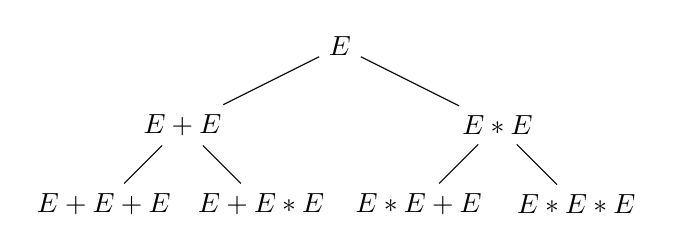
\begin{tikzpicture}[level distance=1cm,
  		level 1/.style={sibling distance=4cm},
  		level 2/.style={sibling distance=2cm}]
  		\node {$E$}
    		child {node {$E+E$}
      		child {node {$E+E+E$}}
      		child {node {$E+E \ast E$}}
    		}
    		child {node {$E \ast E$}
    			child {node {$E \ast E+E$}}
      		child {node {$E \ast E\ast E$}}
    		};
\end{tikzpicture}
\caption{Voorbeeld van een bewerkingsboom} \label{fig:vbBoom}
\end{figure}

Aangezien de groei van de boom exponentieel is, bekomt men zeer grote berekeningstijden om de lagere dieptes van de boom te berekenen. Deze groei valt samen met de toename van de diepte in de boom. Het opstellen van de boom veroorzaakt een grote rekenkost. Dit heeft tot gevolg dat het ten zeerste aangeraden is om deze boom slechts \'e\'enmaal op voorhand uit te werken.

\subsection{Subhypothesen} \label{ssec:subhypothesen}
\par Hieronder vindt u een oplijsting van de subhypothesen:

\begin{itemize}
\item Subhypothese 1: Er zijn redundante knopen in de originele boom.
\item Subhypothese 2: Toevoeging van constanten aan de regels van de contextvrije grammatica heeft een positieve invloed op het vinden van mogelijke vergelijkingen.
\item Subhypothese 3: Er bestaat een optimale afweging tussen de oplossingsgraad en de benodigde tijd bij het toevoegen van constanten.
\item Subhypothese 4: Het vermijden van redundante uitwerkingen heeft een positieve invloed op de tijd. 
\end{itemize}

\subsection{Evaluatiecriteria}

Snelheid, correctheid, gebruikersgemak en uitbreidbaarheid zijn de vier evaluatiecriteria waarop het onderzoek gaat beoordeeld worden. Het doel van het onderzoek is dus een effici\"ent, correct en gemakkelijk uitbreidbaar algoritme te bepalen dat uit een gegeven set van voorbeelden een geschikte vergelijking kan vinden. Ook het gebruikersgemak is van belang.
\end{document}